% Options for packages loaded elsewhere
\PassOptionsToPackage{unicode}{hyperref}
\PassOptionsToPackage{hyphens}{url}
%
\documentclass[
]{book}
\usepackage{lmodern}
\usepackage{amssymb,amsmath}
\usepackage{ifxetex,ifluatex}
\ifnum 0\ifxetex 1\fi\ifluatex 1\fi=0 % if pdftex
  \usepackage[T1]{fontenc}
  \usepackage[utf8]{inputenc}
  \usepackage{textcomp} % provide euro and other symbols
\else % if luatex or xetex
  \usepackage{unicode-math}
  \defaultfontfeatures{Scale=MatchLowercase}
  \defaultfontfeatures[\rmfamily]{Ligatures=TeX,Scale=1}
\fi
% Use upquote if available, for straight quotes in verbatim environments
\IfFileExists{upquote.sty}{\usepackage{upquote}}{}
\IfFileExists{microtype.sty}{% use microtype if available
  \usepackage[]{microtype}
  \UseMicrotypeSet[protrusion]{basicmath} % disable protrusion for tt fonts
}{}
\makeatletter
\@ifundefined{KOMAClassName}{% if non-KOMA class
  \IfFileExists{parskip.sty}{%
    \usepackage{parskip}
  }{% else
    \setlength{\parindent}{0pt}
    \setlength{\parskip}{6pt plus 2pt minus 1pt}}
}{% if KOMA class
  \KOMAoptions{parskip=half}}
\makeatother
\usepackage{xcolor}
\IfFileExists{xurl.sty}{\usepackage{xurl}}{} % add URL line breaks if available
\IfFileExists{bookmark.sty}{\usepackage{bookmark}}{\usepackage{hyperref}}
\hypersetup{
  pdftitle={Technology},
  pdfauthor={Dyrehaugen Web Notebook},
  hidelinks,
  pdfcreator={LaTeX via pandoc}}
\urlstyle{same} % disable monospaced font for URLs
\usepackage{longtable,booktabs}
% Correct order of tables after \paragraph or \subparagraph
\usepackage{etoolbox}
\makeatletter
\patchcmd\longtable{\par}{\if@noskipsec\mbox{}\fi\par}{}{}
\makeatother
% Allow footnotes in longtable head/foot
\IfFileExists{footnotehyper.sty}{\usepackage{footnotehyper}}{\usepackage{footnote}}
\makesavenoteenv{longtable}
\usepackage{graphicx}
\makeatletter
\def\maxwidth{\ifdim\Gin@nat@width>\linewidth\linewidth\else\Gin@nat@width\fi}
\def\maxheight{\ifdim\Gin@nat@height>\textheight\textheight\else\Gin@nat@height\fi}
\makeatother
% Scale images if necessary, so that they will not overflow the page
% margins by default, and it is still possible to overwrite the defaults
% using explicit options in \includegraphics[width, height, ...]{}
\setkeys{Gin}{width=\maxwidth,height=\maxheight,keepaspectratio}
% Set default figure placement to htbp
\makeatletter
\def\fps@figure{htbp}
\makeatother
\setlength{\emergencystretch}{3em} % prevent overfull lines
\providecommand{\tightlist}{%
  \setlength{\itemsep}{0pt}\setlength{\parskip}{0pt}}
\setcounter{secnumdepth}{5}
\usepackage{booktabs}
\usepackage{amsthm}
\makeatletter
\def\thm@space@setup{%
  \thm@preskip=8pt plus 2pt minus 4pt
  \thm@postskip=\thm@preskip
}
\makeatother

\renewcommand\chaptername{}
\usepackage[]{natbib}
\bibliographystyle{apalike}

\title{Technology}
\author{Dyrehaugen Web Notebook}
\date{2022-12-08}

\begin{document}
\maketitle

{
\setcounter{tocdepth}{1}
\tableofcontents
}
\hypertarget{technology}{%
\chapter{Technology}\label{technology}}


\includegraphics{fig/zelda.jpg}

\hypertarget{airplanes}{%
\chapter{Airplanes}\label{airplanes}}

\hypertarget{hydrogen-powered-airplanes}{%
\section{Hydrogen Powered Airplanes}\label{hydrogen-powered-airplanes}}

\emph{Galluchi}

About one-third of total passenger traffic worldwide could be carried by planes burning liquid hydrogen, based on 2019 route data according to a \href{https://theicct.org/publication/aviation-global-evo-hydrogen-aircraft-jan22}{white paper}.

In the most optimistic scenario, aircraft powered by \hspace{0pt}``green hydrogen'' --- produced using renewable electricity --- could reduce total emissions from passenger flights by 31 percent compared to projected emissions levels in 2050.

Aviation contributes about 2.5 percent of global greenhouse gas emissions every year, primarily from burning petroleum-based jet fuel, or kerosene.

Some airlines are already chipping away at their emissions by blending their kerosene with small amounts of \hspace{0pt}``sustainable aviation fuels,'' or SAFs, which are primarily made today from used cooking oils and discarded animal fats. Producers and policymakers are pushing to drastically \href{https://www.canarymedia.com/articles/air-travel/how-do-we-clean-up-air-travel-fuel-from-fast-food-grease-is-just-the-start}{boost adoption} of SAFs for commercial flights starting this decade, from about 26 million gallons every year to several billion gallons a year by 2030.

Yet while plant- and waste-based alternatives can be cleaner to produce than jet fuel, they still emit carbon dioxide when burned in engines. Hydrogen does not --- hence the industry's intensifying efforts to develop H2-powered aircraft.
Hydrogen planes could capture a huge share of shorter flights, but not long trips.

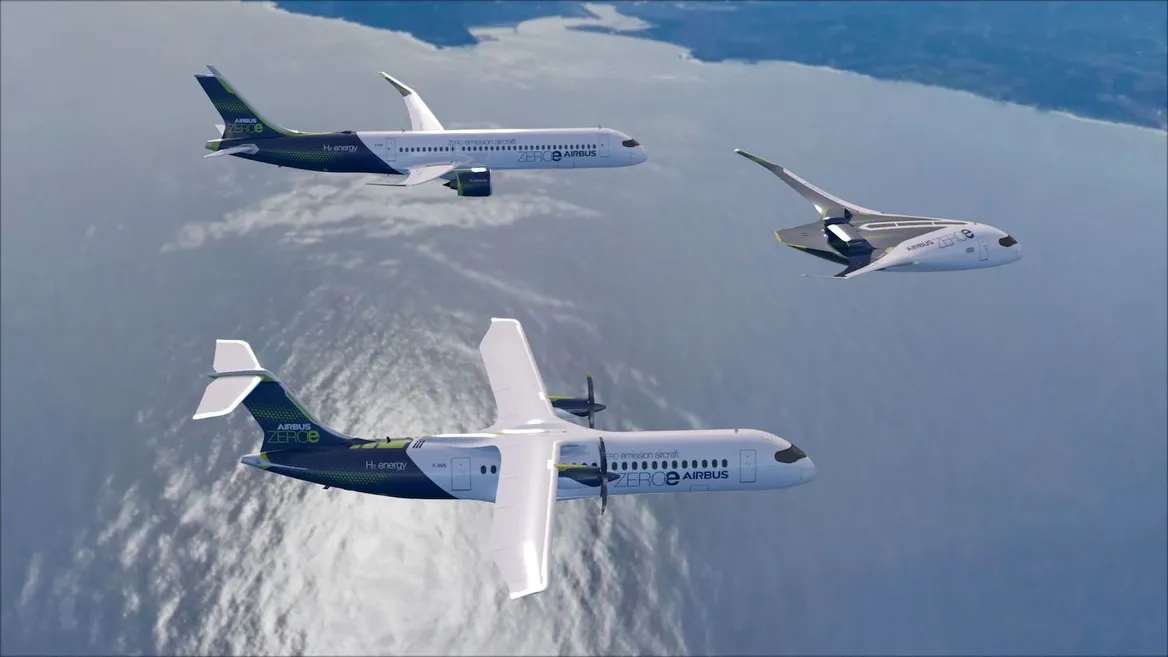
\includegraphics{fig/airbus_hydrogen_concept.png}

\emph{Figure: Airbus Concept Planes}

Liquid hydrogen-powered aircraft would be less energy-efficient and have a shorter range than their kerosene-powered counterparts --- making them impractical for long-haul flights without more technology innovations. However, the zero-emission planes could still service a sizable share of passenger air travel.

A turboprop burning liquid hydrogen could transport 70 passengers up to 1,400 kilometers.
A narrow-body aircraft could carry 165 passengers up to 3,400 kilometers.
Hydrogen planes could service about 97 percent of the turboprop market and 71 percent of the narrow-body market.

Liquid hydrogen packs much less energy on a volume basis than kerosene does, so planes would have to store more of it to travel the same distance. The zero-carbon fuel must also be kept at around -250 degrees Celsius
in heavy cryogenic tanks, further weighing down the plane. In the two Airbus designs, the main bodies of the planes are elongated to accommodate the extra fuel storage.

The world will need to build gigatons' worth of additional wind, solar and other renewable energy capacity to produce enough green hydrogen to supply a zero-emission aircraft fleet --- as well as to power the energy-intensive process of liquifying that hydrogen.

\textbf{Drop-in Fuels}

``Drop-in'' fuels made of used cooking oil or forest residues represent less than 1 percent of total jet fuel demand. In Europe, aviation officials are pushing to accelerate the production and use of such fuels. The ReFuelEU Aviation proposal introduced last year would require that fuels delivered to European Union airports contain at least 2 percent SAF by 2025, ratcheting up to 63 percent by midcentury.

\href{https://www.canarymedia.com/articles/air-travel/hydrogen-powered-planes-could-handle-a-third-of-passenger-air-travel-study-finds}{Galluchi (2022) Hydrogen-powered planes could handle a third of passenger air travel}

\hypertarget{blockchain}{%
\chapter{Blockchain}\label{blockchain}}

Blockchain technology, the design of which was originally seen as facilitating an egalitarian, peer-to-peer sharing economy, is not necessarily neutral and apolitical.

\hypertarget{land-registers}{%
\section{Land Registers}\label{land-registers}}

\emph{Daivirt}

\begin{quote}
There is a need for more empirical insights into the ways how blockchain-based property relations create new territories of accumulation and resistance, and intersect with existing legal and political systems.
\end{quote}

This essay explores the abstraction of blockchain as employed for formalizing land rights in emerging economies. Behind the seemingly neutral façade of the technology, diverse aspirational claims and narratives guide its implementation in different societies, shaped by particular histories and socio-political contexts. This highlights the need to explore blockchain-based land registries as distributed knowledge infrastructures, uncovering their broader embeddedness in older, non-digital modalities, and the ``peopled infrastructures'' of informal networks with their histories and cultural repertoires. As digital technologies can facilitate an illusion of enhanced visibility of some elements while obscuring others, I argue that more attention is needed to the role of broader colonial legacies and enduring North-South inequalities that frequently remain backgrounded in the adoption of such technologies.

An increasing number of governments are investigating the prospects of transferring their land registries to blockchain.
Blockchain applications are explored as enabling the formalization of property rights in the countries of the Global South, as well as providing more efficient coordination of real property markets in the Global North. Blockchain registries have several advantages as compared to centralized digital or paper-based databases. Records on blockchain are distributed and verified by a multitude of nodes in a peer-to-peer digital network, affording them more transparency and resilience. As new additions to the chain of blocks are cryptographically time-stamped, this makes tampering or accidental data loss less likely. Auto-executing ``smart contracts'' that transform legal agreements into code could mediate contracts

Blockchain-based digitalization of land records should be viewed within a broader framework of land tenure formalization in the Global South, where land titling has been advocated as enabling economic development by turning land into tradable asset and a source of credit. Contrary to the expectations of the proponents of neoliberal land reforms, recent land titling initiatives in Africa and Latin America have fueled speculative investment and land concentration.

Many communities in the Global South follow local, alternative rules of property, where land is held under customary tenure and managed as part of a complex system of obligations and debts within a broader kin or territorial group. Reforms that introduce exclusive land rights may exacerbate political conflicts especially in unstable and transitional settings.

\href{https://developingeconomics.org/2021/05/20/land-property-technology-interrogating-an-infrastructural-promise/}{Daivirt (2021) Land, property, technology: interrogating an infrastructural promise}

\hypertarget{carbon-capture}{%
\chapter{Carbon Capture}\label{carbon-capture}}

\hypertarget{low-scale-carbon-capture}{%
\section{Low Scale Carbon Capture}\label{low-scale-carbon-capture}}

\emph{CarbonQuest}

The room-sized CO2 filtration and liquefaction system, installed early this year by CarbonQuest, is a rare instance of carbon capture that actually works and delivers an economic payback. Power-plant or industrial-scale carbon capture has a long history of disappointing results.

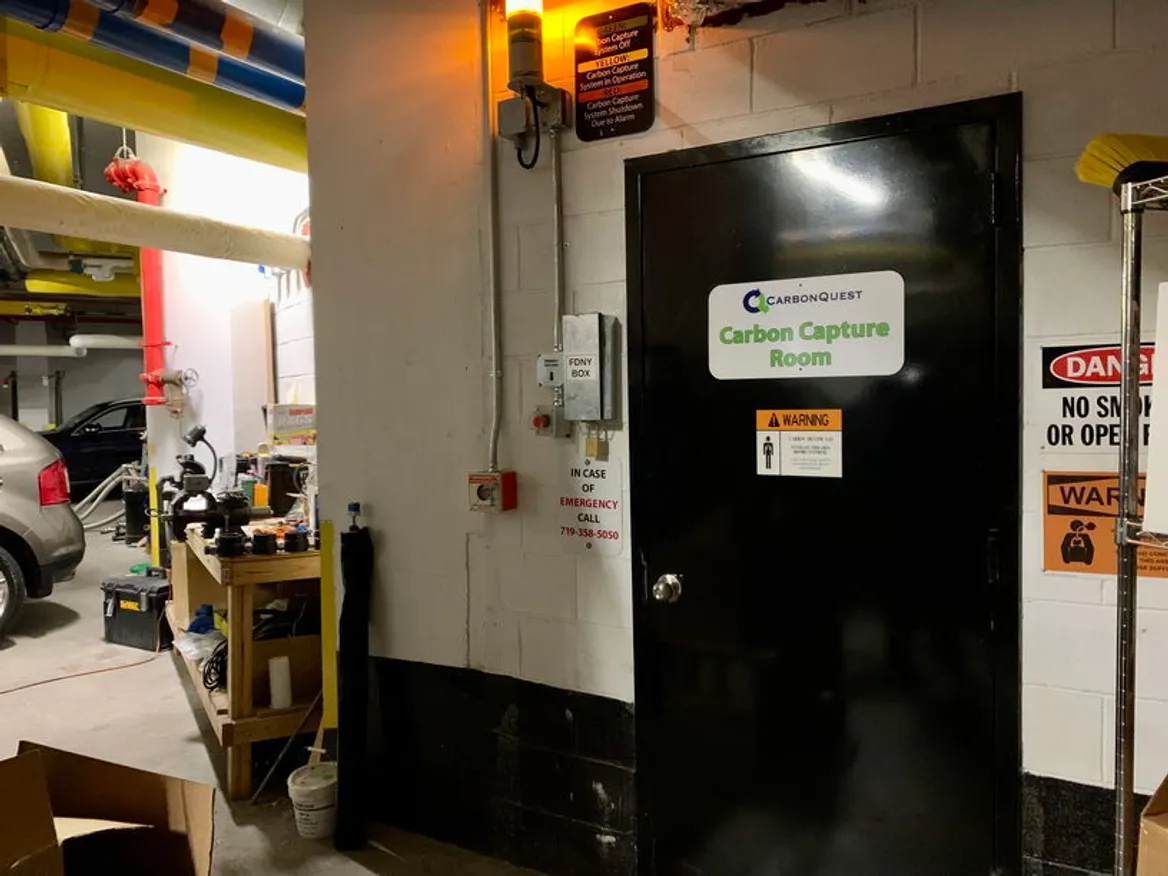
\includegraphics{fig/carbon_capture_room.png}

CarbonQuest captures emissions from existing heating systems, paying back the investment by avoiding penalties under New York's carbon-reduction rules and selling industrial-grade CO2 to paying customers.

CarbonQuest had tapped into the insulated duct that carries hot boiler exhaust to the chimney, diverting the flow through a circuitous array of hissing, humming machinery that pulls out moisture and isolates the carbon dioxide from nitrogen and oxygen, which get released back out the flue.

The carbon dioxide then gets cooled to a liquid state and stored, under pressure, in a metal tank. Eventually, a truck pulls up on the street outside, connects a hose to a nozzle on the side of the building and sucks out the liquid carbon for delivery to a concrete factory, which will inject the greenhouse gas into concrete blocks, making them stronger.

At its current scale, it catches 60 percent of the entire building's gas emissions.

\href{https://www.canarymedia.com/articles/carbon-capture/carbon-capture-for-new-york-high-rise-apartments-is-a-real-thing-now}{Spector (2022) Carbon capture for New York high-rise apartments is a real thing now}

\hypertarget{concrete}{%
\chapter{Concrete}\label{concrete}}

We live in a world of concrete. After water, it's the most widely used substance on our planet, and its usage around the world, ton for ton, is twice that of steel, wood, plastics and aluminium combined.

Its invention in 1824, by a bricklayer in Leeds who first produced the Portland cement used to bind the aggregates used in concrete, quite literally paved the way for the creation of the modern world, enabling humans to mould high-strength, stone-like structures of almost any shape.

Concrete's ubiquity comes at a high price though: if the cement industry were a country, it would be the third-largest emitter of carbon dioxide in the world, after the US and China, as it releases over 2.8 billion tonnes into the atmosphere each year.

A 2018 report suggested concrete contributes up to 8 per cent of the world's CO2 emissions.

It also requires phenomenal amounts of water, sucking up around a tenth of all water used in industry -- often in areas with critical water shortages.

\href{https://www.independent.co.uk/climate-change/news/wood-construction-concrete-steel-climate-b1796342.html}{Cockburn}

\textbf{Major construction firms team up to get the carbon out of concrete}

\emph{Canary Media}

Engineers and architects can reduce the proportion of cement in a number of ways.
One is to use higher-quality aggregate that imparts more structural integrity to the concrete that's made with it.

Another is by using what's called \hspace{0pt}``supplementary cementitious materials'' to replace a portion of the cement used in different mixes of concrete. Fly ash from coal plants and slag from steel mills are the most common alternatives and are being put to use by some major cement and concrete companies such as Cemex. But rice husks, ground glass and several other alternatives can replace anywhere from 10 to 40 percent of the cement.

\href{https://www.canarymedia.com/articles/clean-industry/major-construction-firms-team-up-to-get-the-carbon-out-of-concrete}{Canary media (2022) Major construction firms team up to get the carbon out of concrete}

\hypertarget{growing-limestone-from-algae}{%
\section{Growing limestone from algae}\label{growing-limestone-from-algae}}

\emph{Simpkins}

To make portland cement, the most common type of cement, limestone is extracted from large quarries and burned at high temperatures, releasing large amounts of carbon dioxide.
Replacing quarried limestone with biologically grown limestone, a natural process that some species of calcareous microalgae complete through photosynthesis (just like growing coral reefs), creates a net carbon neutral way to make portland cement. In short, the carbon dioxide released into the atmosphere equals what the microalgae already captured.

\href{https://www.colorado.edu/today/2022/06/23/cities-future-may-be-built-algae-grown-limestone}{Simpkins (2022) Cities of the future may be built with algae-grown limestone}

\hypertarget{mud-constructions}{%
\section{Mud Constructions}\label{mud-constructions}}

\emph{Lewis}

Concrete's heat-retaining properties are all wrong for the Senegalese climate.
Yet concrete has become the ``traditional'' building material in a country.

At least four distinctive mud-construction techniques persist. In the north, where there's not much rain, people build houses with banco, a kind of adobe made with sun-dried bricks; in the forested areas of the south, builders use timber frames to create wattle-and-daub structures, or they hand-mold earthen buildings and top them with steep, overhanging roofs to keep rain away from the walls. For generations, Senegalese builders have used mud to construct not only small houses and granaries but multistory houses and imposing mosques.

Raw-earth-based building materials, such as adobe, rammed earth, and the compressed-earth blocks have more thermal inertia than concrete, which means they attenuate heat and cold more efficiently and reduce the need for so much air-conditioning.

Resistance to mud construction in modern Senegal goes beyond practical concerns: Earth-based materials are widely considered a symbol of poverty, a last recourse for those with no other shelter.

The accessibility of air-conditioning has created a kind of architectural laziness, because buildings no longer need to rely on design to stay cool.

In the nearby village of Ngawlé, Ousmane Mbodj and his family invited me into their \emph{banco} house, and as soon as I stepped inside, my body relaxed. I had no instruments to measure the difference in temperature, but the change felt like a balm.
Thick walls provide natural insulation from the sun, while the limited number of small windows helps the interior stay cool. Outside, thatch-covered verandas or perforated walls create shade and can be used as exterior rooms.

Roof leaks during the rainy season because the local mice like to eat its mud and hay.

In the center of Podor, the local département is constructing a mud-brick administrative building using the Nubian-vault technique. Originating from ancient Egypt, the method uses arches to create self-supporting adobe structures. The technique was revived in the 1940s by the Egyptian architect Hassan Fathy, who attempted to create a whole village of Nubian-vault structures on the banks of the Nile River. That project was never completed, but his approach, which he documented in his book Architecture for the Poor, created new interest in mud construction across the globe. In 2000, a French nonprofit called the Nubian Vault Association streamlined the technique and started training workers to employ it throughout West Africa---starting in Burkina Faso and expanding to Mali, Benin, Ghana, and Senegal.

An earth-construction boom is happening along the sunny coast south of Dakar. Here, earth construction is chosen not just by those with modest budgets and few other options, but by wealthier families with a taste for innovation and bespoke designs.

They had planned to build nearly 12-inch-thick walls for their thermal advantages, but the small lot could only accommodate 9-inch-thick walls. To make up for the difference, they positioned each row of blocks so that it protruded slightly over the row below it, resulting in walls that essentially create their own shade. The walls' textured surface gives them a unique appearance---a style inspired by substance. Though houses like this are far too expensive for most, it illustrates both the practical and aesthetic advantages of mud construction.

Show people that we can build with local materials that will be much more comfortable and much cheaper than concrete.

\href{https://www.theatlantic.com/science/archive/2022/07/senegal-dakar-construction-mud-architecture/661405/}{Lewis (2022) The Future of Mud}

\hypertarget{military-technology}{%
\chapter{Military Technology}\label{military-technology}}

\emph{Smith}

Military technology is a hugely important area of innovation, and yet it generally results in things getting blown up and society going to hell for a while.
Also worrying is how many of the new military technologies are specialized for use off the battlefield.

In 2014, I wrote a post in which I argued that drone dominance of the battlefield would change human society forever:

\begin{verbatim}
[I]magine yourself back in 1400. In that century (and the 10 centuries before it), the battlefield was ruled not by the infantryman, but by the horse archer—a warrior-nobleman who had spent his whole life training in the ways of war. Imagine that guy’s surprise when he was shot off his horse by a poor no-count farmer armed with a long metal tube and just two weeks’ worth of training. Just a regular guy with a gun.

That day was the end of the Middle Ages and the beginning of modernity. For centuries after that fateful day, gun-toting infantry ruled the battlefield. Military success depended more and more on being able to motivate large groups of (gun-wielding) humans, instead of on winning the loyalty of the highly trained warrior-noblemen. But sometime in the near future, the autonomous, weaponized drone may replace the human infantryman as the dominant battlefield technology. And as always, that shift in military technology will cause huge social upheaval.
\end{verbatim}

Six years later, I watched my vision come true. In the Second Nagorno-Karabakh War, Azerbaijan used drones --- purchased cheaply and easily from Turkey and Israel --- to crush the vaunted Armenian army in a short space of time. Armenian troops were renowned as masters of infantry warfare and heavy weaponry, but their tanks, missile launchers, artillery, and transport vehicles were sitting ducks for their foes' cheap disposable drones. No matter how well they concealed their vehicles, the drones could easily spot and destroy them. You can see the incredible toll catalogued at the blog Oryx, with full documentation of each destroyed vehicle.

This should be as big a wakeup call as the Battle of Taranto or the firebombing of Guernica. Drones have changed warfare.

Unless electronic countermeasures or directed energy weapons become very good, very fast, drones will scour the battlefield of human-controlled heavy weaponry at a very low cost, with little risk of life. And they create another battlespace to be fought over --- the low-altitude air, where traditional piloted aircraft no longer go (for fear of being shot down), where radars have trouble spotting threats.

Already countries are racing to build or buy cutting-edge drone systems; this is a true arms race. But we won't know who wins that race unless and until there is a major war.

But the real transformative drone technology might still be in its infancy.

The drones that won the war for Azerbaijan are traditional fossil fuel powered aircraft. Advances in Li-ion batteries have given rise to small, cheap, difficult-to-see, difficult-to-shoot quadcopters. Already, militaries are finding creative uses for these: The IDF (Israel Army) has been using drones to drop tear gas on protesters in Ramallah and the West Bank.

Another example is the UK, whose air force is \href{https://www.thedrive.com/the-war-zone/36950/raf-tests-swarm-loaded-with-britecloud-electronic-warfare-decoys-to-overwhelm-air-defenses}{testing networked swarms of drones} to overwhelm radar systems.

The disturbing possibility is that nations might simply exist in a state of low-grade cyberwarfare at all times, attempting to disable each other's infrastructure.

What COVID-19 made people realize was that you don't need to create some super-deadly virus in order to severely disrupt a society. All you need is a very contagious disease with a mortality rate high enough to scare people. If you're a very very unscrupulous country, you could surreptitiously vaccinate most of your population against this disease and then unleash it on the world.

\href{https://www.americansecurityproject.org/crispr-is-making-bioweapons-more-accessible/}{Crispr technology} and \href{https://cen.acs.org/biological-chemistry/synthetic-biology/Synthetic-biology-enable-bioweapons-development/96/i26}{DNA synthesis}, which are increasingly available to the public, might conceivably create a lot of weird bioweapons that act very differently to the viruses we're used to.

Most of the modern military technologies led themselves to a very different kind of great-power war --- a war of constant sniping and harassment. Assassin drones, cyberattacks, info ops, and bioweapons raise the possibility of never-ending low-grade attacks that are below the threshold of massive retaliation.

To forestall this, military strategists should try very hard to think of new, robust, sophisticated methods of deterrence. Deterrence is the key to peace; it's risky, but when it's successful, it makes military technology act as a protector of human life rather than a destroyer of it. If new technology makes deterrence impossible, it might condemn us to a future where everyone is always on the offense.

\href{https://noahpinion.substack.com/p/the-future-of-war-is-bizarre-and}{Noah Smith}

\hypertarget{shipping}{%
\chapter{Shipping}\label{shipping}}

\hypertarget{windships}{%
\section{Windships}\label{windships}}

\emph{Gallucci}

This year's forecast for the global maritime industry looks particularly breezy. Sails, kites, wings and tubes are all set to appear on cargo vessels over the course of 2022, harnessing wind energy to reduce ships' use of dirty diesel fuels. Experts count nearly two dozen new projects in the works as shipping companies look to limit emissions from carrying cargo by sea.

\href{https://www.canarymedia.com/articles/sea-transport/sailing-into-2022-with-wind-powered-cargo-ships}{Gallucci (2022) Sailing into 2022 with wind-powered cargo ships}

\hypertarget{social-media}{%
\chapter{Social Media}\label{social-media}}

\hypertarget{twitter}{%
\section{Twitter}\label{twitter}}

\emph{Noahpinion}

\textbf{Dimensions}

Two years ago, my friend Eugene Wei wrote a blog post called \href{https://www.eugenewei.com/blog/2019/2/19/status-as-a-service}{``Status as a Service (Staas)''}, which laid out what has become the canonical framework for thinking about social media. Eugene basically divides social media's function into three dimensions --- utility (i.e., direct usefulness), entertainment value, and social capital. He spends much of the post discussing the third of these --- the way social networks create new ways for people to gain status and respect. Get the most Twitter follows, or the most Facebook likes, etc., and you're somebody. Social media has democratized celebrity; anyone can be an influencer.

Anyone, but not \emph{everyone}. Just as most people can't become Hollywood stars, most people can't become social media influencers. But unlike in the old days, when people would obsess over Hollywood actors from afar, nowadays social media allows people to come in contact with their heroes directly. And no network facilitates this more than Twitter.

I continue to believe that Twitter, alone among all social networks created thus far, represents something truly new under the sun. Facebook and LinkedIn more-or-less preserves the networks of personal friendship, hobby interest, and professional networking that exist offline. Instagram maintains the celebrity-fan dynamic, with influencers dominating their pages at an Olympian remove. But on Twitter, anyone can talk directly to anyone at any time, and, short of blocking them, the person they're talking to can't stop you from talking to them.

On other social networks, if you created a post, you can delete comments that you don't like; you are the moderator of your own threads. But on Twitter you can't. There is a ``hide replies'' function, but it just sends the replies to a special ``hidden replies'' section where anyone can peruse them at will. Even if you block someone who replies to you, their reply-tweet remains.

These two quirks of Twitter --- free direct communication and no ability to regulate replies --- make all the difference. Suddenly, people can talk directly to any celebrity, any politician, any journalist or activist or influencer of any kind. And the person they're talking to can't stop them.

Being able to reply to high-status people, whether they want you to or not, is a heady status-conferring experience. You can say mean shit to the most famous Hollywood movie star, and there's nothing he can do about it. Or you can say something nice, and hopefully get a reply or a shout-out. This puts you on a plane of near-equality with people who otherwise tower over the social landscape.

Near-equality, but not equality!
This can be maddening. Twitter creates the instantaneous illusion of social equality between influencers and normal people.

That process, which repeats itself many millions of times every day, creates some very unusual social dynamics. For example, there's ``the ratio'', in which a mob of reply-tweeters try to leave someone with more replies than likes. It feels heady to be part of a ratio-mob, as evidenced by the people who reply with ``just here for the ratio'', or who re-state a rebuttal that many others have already made. (Some people have invented a second type of ``ratio'' that doesn't depend on being part of a mob: writing a reply-tweet that gets more likes than the original tweet it's replying to. I've seen Zoomers in group chats bragging about the famous people they managed to ``ratio'' this way.)

By bringing people much closer together in social status, Twitter emphasizes the intractable gaps that remain.

As Twitter ages and the distribution of status gets even more frozen in, Twitter will have to rely on status anxiety more and more to keep new users engaged.
They've never taken the crucial step of allowing people to actually drop reply-tweets from their threads or untag themselves from other people's tweets. Doing that might make Twitter a lot nicer of a place

Thus, Twitter will continue to be the place where Americans go to scream at strangers --- where status is conferred not just by little snippets of viral pseudo-wisdom, but by the ability to ridicule and attack those snippets. We should probably think long and hard about whether it's a good idea to have our public discourse dominated and directed by a platform with that basic dynamic.

\href{https://noahpinion.substack.com/p/status-anxiety-as-a-service}{Noahpinion (2021) Status Anxiety as Service}

\hypertarget{steel}{%
\chapter{Steel}\label{steel}}

Today, the U.S. only accounts for about 5 percent of global steel production capacity.

If the U.S. is to achieve Biden's vision of a new deal for America, complete with infrastructure upgrades, domestically sourced materials and net-zero emissions, the country needs not only to reverse its flagging fortunes in the steel market but also to foster new technologies that will enable it to produce ``green'' steel with a minimum of carbon dioxide emissions. Such new technologies are now under development, although their entry into the marketplace is going to require time, investment and government support.

Steel production is one of humanity's most environmentally destructive activities. Even in its diminished state, the U.S. steel industry releases more carbon dioxide emissions than any other domestic industry --- nearly a ton of carbon dioxide for every ton of steel produced.

That's largely because steel-making relies on coal and natural gas for most of its hefty energy consumption.

Steel industry emissions must be mitigated at first by eking out small improvements to a wide variety of production stages. Simply using steel more efficiently is the first step. For example,
some \href{https://energycentral.com/c/ec/new-innovation-drives-down-carbon-dioxide-emissions-cement}{new forms of concrete} are structurally stable without the use of steel reinforcing bars. Also, other materials can be substituted for steel;
one young company called \href{https://www.inventwood.com/}{Inventwood} is developing a process that transforms wood into \href{https://www.inventwood.com/mettlewood/}{a material strong enough to be used in place of steel}.

Another technique is to recycle more steel. According to the International Energy Agency, producing steel from recycled scrap requires only one-eighth the energy associated with producing steel from iron ore. Scrap accounts for about 70 percent of the raw metal input to U.S. steel production today, a figure that can be boosted.

But that alone won't obviate the need for new steel mills, since future demand for steel will outpace past supply. Instead, the U.S. will have to make new steel from iron ore and mitigate the emissions stemming from that process.

To better understand the options for improvement, let's review how steel is typically made. First, iron ore and fossil fuels (usually either specially refined coal or natural gas) are put in a furnace, where the fuels are burned to produce heat, carbon monoxide and carbon dioxide. The carbon monoxide combines with oxygen from the iron oxide contained in the ore, forming carbon dioxide and leaving behind a quantity of nearly pure iron. That iron is then conveyed either to a specially lined vat where oxygen is blown through liquid iron or to an electric furnace. In these secondary vessels, the iron is further purified and combined with small amounts of carbon to make steel.

One way to mitigate the carbon emissions from this process is to capture carbon dioxide from the furnace and sequester it in underground reservoirs.
Most carbon-capture facilities don't actually sequester the carbon dioxide they capture. Instead, they sell it to oil companies that then pump it underground to force oil to the surface, a process known as enhanced oil recovery (EOR).
The only operating steel plant using carbon capture at scale, the Al Reyadah plant in Abu Dhabi, employs this technique.
It's not clear that EOR sequestration actually reduces emissions on a net basis if the calculation includes the carbon dioxide released by burning the oil that's produced.
It's unlikely this technique will result in significant reductions of net emissions.

Other techniques include improving the efficiency of the ore processing furnaces and replacing coal furnaces with natural-gas furnaces. These techniques will only provide marginal emission reductions.

\textbf{New steel-making technologies}

\textbf{\emph{H2 DRI}}

The two leading steel-making technologies with the potential to nearly eliminate carbon dioxide emissions use a common chemical process known as electrolysis.

One technology that's well on its way is called ``hydrogen direct reduced iron'' (H2 DRI). It is now being demonstrated in Sweden, Japan and Germany. H2 DRI substitutes hydrogen (preferably, but not necessarily, made with clean energy) for the coal or natural gas used in the typical furnace process. In a DRI furnace, the iron ore is heated but not to the point of melting. Hydrogen then passes over the hot ore, combining with oxygen liberated from the iron oxide to form water and leaving relatively pure iron behind. Typically, that still-hot iron is then transferred to an electric furnace for additional processing to turn it into steel. If the electricity used to produce the hydrogen and run the furnace comes from non-carbon-emitting sources, then the overall process results in little to no carbon dioxide emissions.

In Sweden, a joint venture dubbed Hybrit (comprising utility Vattenfall, iron ore processor LKAB and steel maker SSAB) is running a pilot H2 DRI plant. This spring, it started to use hydrogen produced via electrolysis from electricity generated by fossil-free sources. (This being Sweden, those probably consist of nuclear and hydropower, with a bit of wind power sprinkled in.) Building a full-scale H2 DRI plant, including electrolyzers to produce hydrogen from clean electricity, costs billions of dollars, and the process consumes prodigious amounts of electricity. Its economics strongly depend on the cost of that electricity and the value of the avoided carbon dioxide emissions. According to the consultancy McKinsey, H2 DRI is not expected to be cost-effective in Europe until sometime between 2030 and 2040.

\textbf{\emph{MOE}}

The other technology under development, molten oxide electrolysis (MOE), also employs electrolysis. But in this case, it's applied directly to the iron oxide ore by placing it in an electrolytic cell filled with a mineral-bearing solution. An electric current is run through the solution, heating it up beyond the melting point of iron, and separating oxygen from iron. If the electricity used to power the MOE process comes from clean sources, the steel can be made with virtually no carbon dioxide emissions.

In the U.S., MOE is being developed by Boston Metal, a company spun out of the Massachusetts Institute of Technology. Like H2 DRI, MOE economics are heavily dependent on the cost of clean electricity. Boston Metal is currently gearing up to build its first pilot plant in Massachusetts, and it is looking into building a larger facility in Quebec or another location with cheap hydroelectricity.

\emph{Prospects}

Of the two technologies, H2 DRI is clearly further along, with a pilot plant in operation and a full-scale plant in development. MOE has some intriguing advantages for the U.S. market, however. First, it's more efficient, requiring somewhere between 15 and 30 percent less electricity than H2 DRI per ton of steel output. Second, MOE facilities can be constructed in much smaller increments than H2 DRI, although exactly how small isn't clear just yet. That's a big deal in the U.S., where a diminished steel industry is unlikely to invest billions of dollars for a new steel plant based on new technology.

Furthermore, Boston Metal's electrolysis cells are so clean that developers would have far more flexibility in where they're located. For example, they could be placed near inexpensive sources of clean electricity or iron ore, or maybe even in Pittsburgh. Both technologies are going to take at least a decade before they're ready to start claiming significant amounts of market share, but over the long run, the odds of Boston Metal's MOE technology gaining traction in the U.S. market appear to be better.

Because steel constitutes just a small portion of most products of which it's a component, that price premium is likely to be small. For example, the International Energy Agency estimates that using green steel would increase the cost of a midsized car by around 0.1\%

\href{https://www.canarymedia.com/articles/joe-bidens-green-new-steel/}{CanaryMedia}

\hypertarget{supply-chain}{%
\chapter{Supply Chain}\label{supply-chain}}

\emph{Smith}

Ocean freight costs alone add 5\% to 10\% to the cost of everything we buy, and remember, 90\% of the stuff we buy is shipped on a container ship. The globalized supply chain and shipping containers have brought down the cost of shipping goods and manufacturing by close to 90\% over the last 50 years.

In America, the ports are owned by the local city that they're in. Therefore, they're not managed as a strategic national asset, which they clearly are.

We've under invested in our supply chain infrastructure for over 20 years.

In hindsight, the signs were there for years. Almost no logistics companies can show you where your freight is in real-time on a map. Most data is exchanged in unstructured email messages with attachments. There are almost no logistics APIs to speak of.

We're going to get sub-optimal outcomes if you don't invest in technology. If we don't have robotics, if we don't have systems that are better at managing appointments for managing pickups and returns of containers at ports, if we don't have better safety mechanisms (some of these are incredibly hazardous jobs and robots would be far safer), it's going to take many years, not months to fix this crisis. Technology and automation have helped modernize and increase the efficiency of ports in other countries like the port of Rotterdam in the Netherlands, but that's because it's managed as a strategic asset for the country. It has been a fully automated operation for over 20 years so the technology exists, but we still have a lack of investment to implement those changes in the United States.

\emph{N.S.: What should the Biden administration have done to overwhelm supply chain bottlenecks early on in the crunch? What should the administration be doing now?}

R.P.: I think many of us imagined that we live in a world where there's a wizard behind the box. That there's actually somebody in charge of all of this, and that that somebody must have made a mistake. And of course, it must be the president of the United States. But that's not actually the world that we live in. It's a market-based system. We're lucky to live in an economy that's built on the principles of free enterprise, and so while it's easy to cast blame and point fingers at the administration, we have to recognize that they're not really in charge of all of these things. They didn't create this situation and I'm not 100\% convinced that they're the ones that are going to be best equipped to solve the problem.

\emph{N.S.: Was the global economy simply over-engineered? Did we optimize supply chains for efficiency at the cost of resilience, like a machine with tolerance gaps that are too small? And if so, should we recalibrate going forward, to leave more slack in the system in case of future crises?}

R.P.: In my opinion, what's caused all the supply chain bottlenecks is modern finance's obsession with Return on Equity (ROE). To show great ROE, almost every CEO stripped their company of all but the bare minimum of assets. ``Just-in-time'' everything with no excess capacity, no strategic reserves, no cash on the balance sheet and minimal investment in R\&D.
We stripped the shock absorbers out of the economy in pursuit of better short-term metrics.
Large businesses are supposed to be more stable and resilient than small ones, and an economy built around giant corporations like America's should be more resilient to shocks. However, the obsession with ROE means that no company was prepared for the inevitable hundred-year storms. Now as we're facing a hundred-year storm of demand, our infrastructure simply can't keep up.
And let's not forget the human aspect of the workforce that makes this all happen. A lot of companies in the industry haven't invested in taking care of their people, especially during market downturns, so now they can't staff up quickly to meet surging demand.

The Dutch government has pushed for infrastructure innovation for decades and has a great working relationship with unions and employers through a \href{https://en.wikipedia.org/wiki/Polder_model}{polder model}, which is based on consensus. This effort was started in the eighties. They used the polder model to successfully implement solutions developed by Delft University of Technology.

There were two reasons they were able to accomplish this:

\begin{itemize}
\item
\begin{verbatim}
      The Port of Rotterdam, a government-owned commercial entity running the port, had this vision way before other countries did as logistics is a key source of GDP in the Netherlands.
\end{verbatim}
\item
\begin{verbatim}
      They had a proper, documented approach to getting buy-in from multiple stakeholders through a polder model. The polder model is a method of consensus decision-making, based on the acclaimed Dutch version of consensus-based economic and social policy making in the 1980s and 1990s. The model is characterized by the cooperation between employers' organizations, labor unions and the government with a central forum to discuss labor issues (with a long tradition of consensus). This model helped them defuse labor conflicts and avoid strikes. Similar models are used in Finland.
\end{verbatim}
\end{itemize}

We should really explore why the U.S. can't do what many mature and rapidly-growing economies already have. Big structural changes are hard to make, but we should at least start somewhere. For example, new technology can be used to eliminate appointments at terminals and allow truck drivers to just show up and take the first available container with a mobile app telling them where to go. We've already built this technology and it's ready to go right now and we believe it could clear the backlog at the Long Beach/Los Angeles ports within 30 days. However, it requires changes to contracts of who's responsible for picking up which container and a lot of coordination between the private sector, trucking companies, importing businesses, warehouses, ports and ocean carriers. This type of coordination is inherently difficult for the private sector to coordinate, where each is looking out for their own best interests.

\href{https://noahpinion.substack.com/p/interview-ryan-petersen-ceo-of-flexport}{Smith (2021) Interview: Ryan Petersen, founder and CEO of Flexport}

\hypertarget{wood}{%
\chapter{Wood}\label{wood}}

Architects and developers are increasingly aware of the role played by steel and concrete manufacturing in the worsening climate crisis, and there is already a move in some quarters towards much more sustainable building materials.

One such material is already being widely used in construction, but recent advances mean it is stronger and more durable than it has ever been before, and has a far, far lower environmental impact than concrete or steel. That material is wood.

Though timber-framed buildings are hardly new, instead of sawing enormous beams from ancient trees, new techniques focus on using fast-growing soft woods, stuck together in a form which provides massive strength, durability, and flexibility of design.

One example of this, cross-laminated timber (CLT), is manufactured using a technique developed in the 1990s in Austria, in which sheets of kiln-dried wood are glued on top of each other, with the grain of each layer running perpendicular to the next.

This method can create huge boards, up to a foot thick, and as long and as wide as the manufacturer's premises allow.

What's more, the strength of these coagulated timber slabs can match or exceed steel or concrete.

The use of CLT as a modern construction material has already been definitively proven.

The world's largest CLT structure is Dalston Works, a 10-storey residential building of 101 flats, in Hackney, London, which was completed in 2017, and won the ``eco living award'' at the Evening Standard's 2018 New Homes Awards.

Meanwhile, the world's tallest timber building has also been built using CLT -- the 85.4-metre, 18-storey Mjostarnet building in Norway, which was completed in 2019 and is also the country's third-tallest building. The mixed-use building contains apartments, a hotel, a swimming pool, office space and a restaurant.

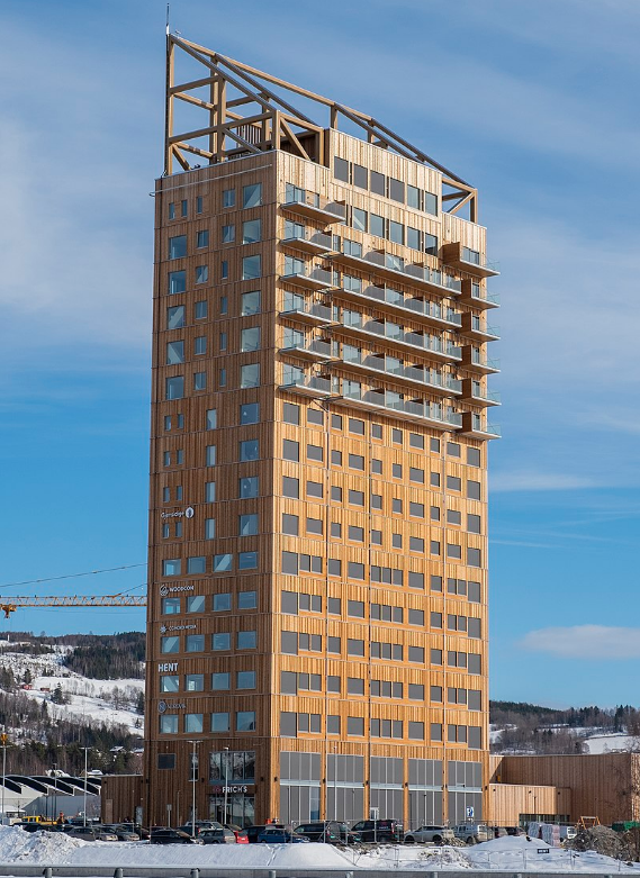
\includegraphics{fig/mjostarnet.png}

\emph{Figure: Mjøstårnet}

For new buildings, the energy regulations are pushing energy consumption and carbon emissions down to the point that the main carbon emissions from new buildings through their life cycle come from their construction and materials.

CLT buildings may be able to store more carbon in the wood than their entire construction generates.

As trees absorb CO2 when they grow, CLT is considered to have a negative embodied carbon -- meaning that the CO2 absorbed by the tree during its growth can be more than that emitted in the manufacture of the CLT product and its transportation to the site.

At the end of its useful life CLT can be repurposed -- something tricky to achieve with other building materials.

The timber used should come from managed forests which have been properly certified as being sustainable sources of wood.

However, ``sustainable forestry'' is a contentious subject, with different meanings in different countries. While vast forests of fast-growing conifers may be able to rapidly fulfil timber orders, a growing understanding of the impact of monoculture cropping on biodiversity, and what it means for carbon sequestration, is also a key consideration for those seeking to herald CLT as a straightforward environmentally friendly choice.

The wood used in the 10-storey Dalston Works building in London was grown in forests in Austria and Germany which have been certified as sustainable.

It was then manufactured into CLT in Austria and brought by road to the UK.

According to the developers, the building used 4,500 cubic metres of timber, which equates to about 2,300 trees. With more than 800 people living in the building, they say it worked out at about three trees per person.

the main tree grown for construction in the UK is the sitka spruce, an imported conifer from the Pacific northwest of North America.

In their home region these trees can reach 40-70 metres in height, but in the UK, where conditions are milder, their growth rate is faster but the resulting density of the wood is lower, making it weaker.

As a result, higher strength timber grown in Europe is normally used for key structural purposes.

One particular concern about the extensive use of wood in construction is the potential for flammability.

In order to be used as a commercial construction material, CLT has been extensively fire-tested, and is designed to accommodate substantial fire resistance.

Furthermore, unlike steel, CLT remains structurally stable when subjected to high temperatures.
CLT is green, cost-effective, fast to install, requires less foundation, and results in less waste than traditional construction.

\emph{From Comments}

It is incorrect to say that CLT ``unlike steel'' remains structurally stable to high temperatures. Steel used in buildings retains at least 100\% of its cold strength up to about 360°°C. (It's actually stronger at around 150-300°C.) What is true is that its insulation properties causes wood to degrade more slowly when exposed to heat as the heat doesn't penetrate so fast. Which is why steam boilers are made out of steel and not wood

\href{https://www.independent.co.uk/climate-change/news/wood-construction-concrete-steel-climate-b1796342.html}{Cockburn}

\hypertarget{science}{%
\chapter{Science}\label{science}}

\hypertarget{science-slowdown}{%
\section{Science Slowdown}\label{science-slowdown}}

\emph{Noah Smith}

\textbf{Low-hanging fruit and the rising cost of science}

The basic idea of science stagnation is that the easiest discoveries happen first. 150 years ago, a monk sitting around playing with plants was able to discover some of the most fundamental properties of inheritance; now, biology labs are gigantic and hugely expensive marvels of technological complexity, and the NIH spends tens of billions of dollars every year. 400 years ago we had people rolling balls down ramps to study gravity; now we study gravity with billion-dollar gravitational wave detectors that require the efforts of thousands of highly trained scientists. And so on.

In 2020, four economists --- Nicholas Bloom, Charles I. Jones, John Van Reenen, and Michael Webb --- published a \href{https://web.stanford.edu/~chadj/IdeaPF.pdf}{paper} quantifying this principle, and the results are deeply disturbing. Across a wide variety of fields, they found that the cost of progress has been rising steadily; more and more researchers (or ``effective researchers'') are required for each incremental advance. This is exactly what a ``low-hanging-fruit'' model of science would predict.

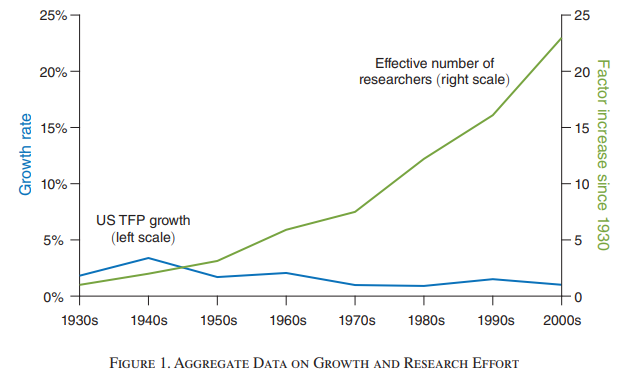
\includegraphics{fig/researchers_TFP.png}

The idea of increasingly expensive research, unlike the other stagnationist arguments I addressed in earlier posts, is very hard to rebut --- the theory is simple and powerful and the data is comprehensive and clear. But there are a few caveats to note here.

Important discoveries become more important as they age. Quantum mechanics was certainly cool stuff back in the 1920s, but it wasn't until later that things like quantum field theory built on it, or engineering applications were developed that made use of it.

Science is progressive like that; each discovery is supported by the discoveries that came before it (in Newton's words, it ``stands on the shoulders of giants''). Thus, each new discovery makes the older discoveries that support it that much more important.

The upshot here is that even if science is getting more expensive, we can still afford to spend more resources and sustain it for a while.

\href{https://www.nber.org/papers/w27863}{Jones and Summers} make a simple model of the economy in which R\&D spending drives growth, plug recent numbers for our real economy into that model, and then ask how much it would reduce growth if we were to stop spending on R\&D. The answer is: A lot.

R\&D is a reliable money-printing machine: you put in a dollar, and you get back out much more than a dollar.

\href{https://mattsclancy.substack.com/p/an-example-of-high-returns-to-publicly}{Clancy} links us to a bit of evidence that R\&D spending still drives progress forward, explaining the results of several papers that find that government research grants to small businesses were very effective at creating patentable inventions in both the U.S. and the EU.

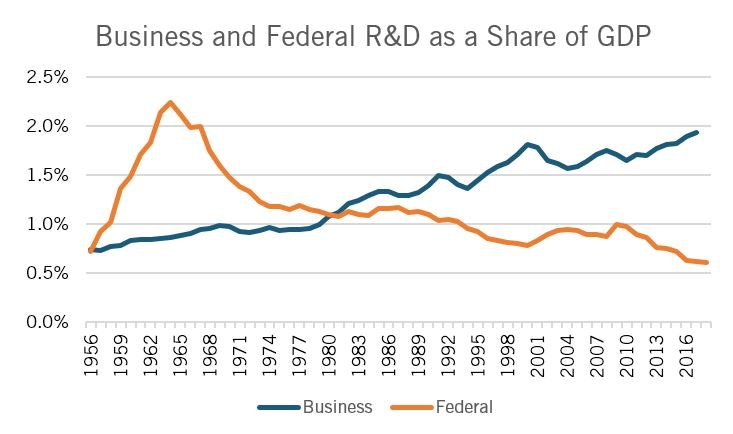
\includegraphics{fig/federal_and_business_RD.jpeg}

Business is running fast enough to stay in place in terms of R\&D, but the government isn't even doing that much.

The upshot of all this is that while the increasing cost of science is a real and significant concern, it doesn't mean it's all stagnation from here on out. We still probably have enough money to accelerate technological progress once again, if we're willing to spend it.

\href{https://noahpinion.substack.com/p/answering-the-techno-pessimists-complete}{Noah Smith (2021)}

\hypertarget{part-appendices}{%
\part{Appendices}\label{part-appendices}}

\hypertarget{appendix-appendices}{%
\appendix}


\hypertarget{about}{%
\chapter{About}\label{about}}


\includegraphics{fig/me.jpg}

\emph{Dyre Haugen} and \emph{Dyrehaugen} is Webian for \emph{Jon Martin} -
self-owned Globian, Webian, Norwegian and Canarian with
a background from industrial research policy, urban planning and
economic development consulting on global, regional and urban scales.
I am deeply concerned about the (insane) way
humanity (i.e.~capitalism) interfere with nature.
In an effort to gain insights in how and why this happens
stuff is collected from around the web and put together
in a linked set of web-sites.
The sites are operated as personal notebooks.
However, these days things can be easily published to the
benefit of others concerned with the same issues.
But be aware - this is not polished for presentation or
peer-reviewed for exactness.
I offer you just to have a look at my `work-desk' as it appears in the moment.
Any comment or suggestion can be mailed to \href{mailto:dyrehaugen@gmail.com}{\nolinkurl{dyrehaugen@gmail.com}}
You can follow me on twitter as @dyrehaugen.
Thanks for visiting!

\hypertarget{links}{%
\chapter{Links}\label{links}}

\textbf{Current Dyrehaugen Sites:}

\begin{itemize}
\tightlist
\item
  \href{https://dyrehaugen.github.io/rcap}{rcap - On Capitalism} \href{http://localhost/rcap}{(loc)}
\item
  \href{https://dyrehaugen.github.io/rclm}{rclm - On Climate Change} \href{http://localhost/rclm}{(loc)}
\item
  \href{https://dyrehaugen.github.io/recs}{recs - On Economics} \href{http://localhost/recs}{(loc)}
\item
  \href{https://dyrehaugen.github.io/rngy}{rfin - On Finance} \href{http://localhost/rfin}{(loc)}
\item
  \href{https://dyrehaugen.github.io/rngy}{rngy - On Energy} \href{http://localhost/rngy}{(loc)}
\item
  \href{https://dyrehaugen.github.io/renv}{renv - On Environment} \href{http://localhost/renv}{(loc)}
\item
  \href{https://dyrehaugen.github.io/rsts}{rsts - On Statistics} \href{http://localhost/rsts}{(loc)}
\item
  \href{https://dyrehaugen.github.io/rurb}{rurb - On Urbanization} \href{http://localhost/rurb}{(loc)}
\item
  \href{https://dyrehaugen.github.io/rvar}{rvar - On Varia} \href{http://localhost/rvar}{(loc)}
\item
  \href{https://dyrehaugen.github.io/rwsd}{rwsd - On Wisdom} \href{http://localhost/rwsd}{(loc)}
\end{itemize}

\textbf{Blogs:}

\begin{itemize}
\tightlist
\item
  \href{https://dyrehaugen.github.io/rde}{rde - Blog in English} \href{http://localhost/rde}{(loc)}
\item
  \href{https://dyrehaugen.github.io/rdn}{rdn - Blog in Norwegian} \href{http://localhost/rdn}{(loc)}
\end{itemize}

\textbf{Discontinued:}

\begin{itemize}
\tightlist
\item
  \href{https://dyrehaugen.github.io/jdt}{jdt - Collection (Jekyll)} \href{http://localhost/jdt}{(loc)}
\item
  \href{https://dyrehaugen.github.io/hdt}{hdt - Collection (Hugo)} \href{http://localhost/hdt}{(loc)}
\end{itemize}

\textbf{Not listed:}

\begin{itemize}
\tightlist
\item
  (q:) dhe dhn jrw56
\item
  (z:) rcsa rpad rstart
\end{itemize}

\hypertarget{news}{%
\chapter{NEWS}\label{news}}

  \bibliography{book.bib,packages.bib}

\end{document}
